\chapter{Modello Cinematico e Simulazione Preliminare} \label{chap:modello}

Questo capitolo descrive la modellistica matematica e la simulazione in catena aperta ("open-loop") del sistema uniciclo a guida differenziale, soddisfacendo gli obiettivi del Punto 1 del progetto. L'analisi si divide in due parti: la formalizzazione del modello affine nel controllo e la validazione sperimentale tramite un test a ingressi variabili a tratti.

\section{Definizione del Sistema}

\subsection{Parametri e Variabili di Stato}
Il sistema è definito dai seguenti parametri geometrici, come da specifiche di progetto:
\begin{itemize}
    \item Raggio delle ruote: \( r_1 = r_2 = 0.10 \) m
    \item Lunghezza asse (carreggiata): \( l = 0.40 \) m
\end{itemize}

Lo **stato del sistema** è rappresentato dal vettore \( z \in \mathbb{R}^3 \):
\begin{equation}
    z = \begin{bmatrix} x \\ y \\ \theta \end{bmatrix}
\end{equation}
con condizione iniziale fissata all'origine: \( z(0) = [0.00; 0.00; 0.00] \).

\subsection{Modello Cinematico}
Il modello cinematico, assumendo condizioni di puro rotolamento e parametri di efficienza nominali (\( w_1 = w_2 = 1.00 \)), è descritto dall'equazione:
\begin{equation} \label{eq:modello_affine}
    \dot{z} = g_1(z)u_1 + g_2(z)u_2
\end{equation}
dove gli ingressi \( u = [u_1, u_2]^T \) sono le velocità angolari delle ruote e i campi vettoriali sono:
\begin{equation}
    g_1(z) = \begin{bmatrix} \frac{r_1}{2}\cos\theta \\ \frac{r_1}{2}\sin\theta \\ \frac{r_1}{l} \end{bmatrix}, \quad
    g_2(z) = \begin{bmatrix} \frac{r_2}{2}\cos\theta \\ \frac{r_2}{2}\sin\theta \\ -\frac{r_2}{l} \end{bmatrix}
\end{equation}

\section{Validazione Sperimentale}
È stato condotto un test di validazione su un orizzonte temporale \( T = 30 \) s, applicando una sequenza di 6 fasi di ingressi costanti a tratti per sollecitare tutte le dinamiche del veicolo (rettilineo, curva, rotazione pura).

\subsection{Protocollo di Test}
La sequenza degli ingressi di controllo applicati è la seguente:
\begin{enumerate}
    \item \textbf{0-5 s (Rettilineo):} \( u = [5; 5] \) rad/s. Avanzamento lungo l'asse x.
    \item \textbf{5-10 s (Curva Sx):} \( u = [6; 4] \) rad/s. Moto curvilineo con raggio di curvatura costante.
    \item \textbf{10-15 s (Rettilineo):} \( u = [5; 5] \) rad/s. Avanzamento in direzione obliqua.
    \item \textbf{15-20 s (Curva Dx):} \( u = [4; 6] \) rad/s. Recupero dell'orientamento.
    \item \textbf{20-25 s (Rettilineo):} \( u = [5; 5] \) rad/s.
    \item \textbf{25-30 s (Rotazione):} \( u = [3; -3] \) rad/s. Rotazione su se stesso (velocità lineare nulla).
\end{enumerate}

\subsection{Analisi dei Risultati}
La simulazione ha prodotto i risultati visibili in Figura \ref{fig:p1_results}. I dati quantitativi finali confermano la correttezza del modello:

\begin{itemize}
    \item \textbf{Stato Finale:} Al termine della simulazione (\( T=30 \) s), il sistema ha raggiunto lo stato:
    \[ z(T) = \begin{bmatrix} 4.19 \, \text{m} \\ 5.10 \, \text{m} \\ 7.50 \, \text{rad} \end{bmatrix} \]
    L'orientamento finale \( \theta \approx 7.50 \) rad (corrispondente a \( 429.72^\circ \)) è coerente con la somma delle rotazioni accumulate nelle varie fasi, in particolare l'ultima fase di rotazione pura che contribuisce significativamente all'incremento angolare.
    
    \item \textbf{Distanza Percorsa:} La distanza totale percorsa dal centro dell'asse è risultata pari a **12.50 m**. Questo valore è consistente con l'integrale della velocità lineare \( v = \frac{r}{2}(u_1+u_2) \) lungo la traiettoria.
    
    \item \textbf{Traiettoria:} Il grafico nel piano XY mostra un percorso a "S" seguito da una sosta in posizione con rotazione continua, rispecchiando fedelmente la sequenza degli ingressi.
\end{itemize}

\begin{figure}[h]
    \centering
    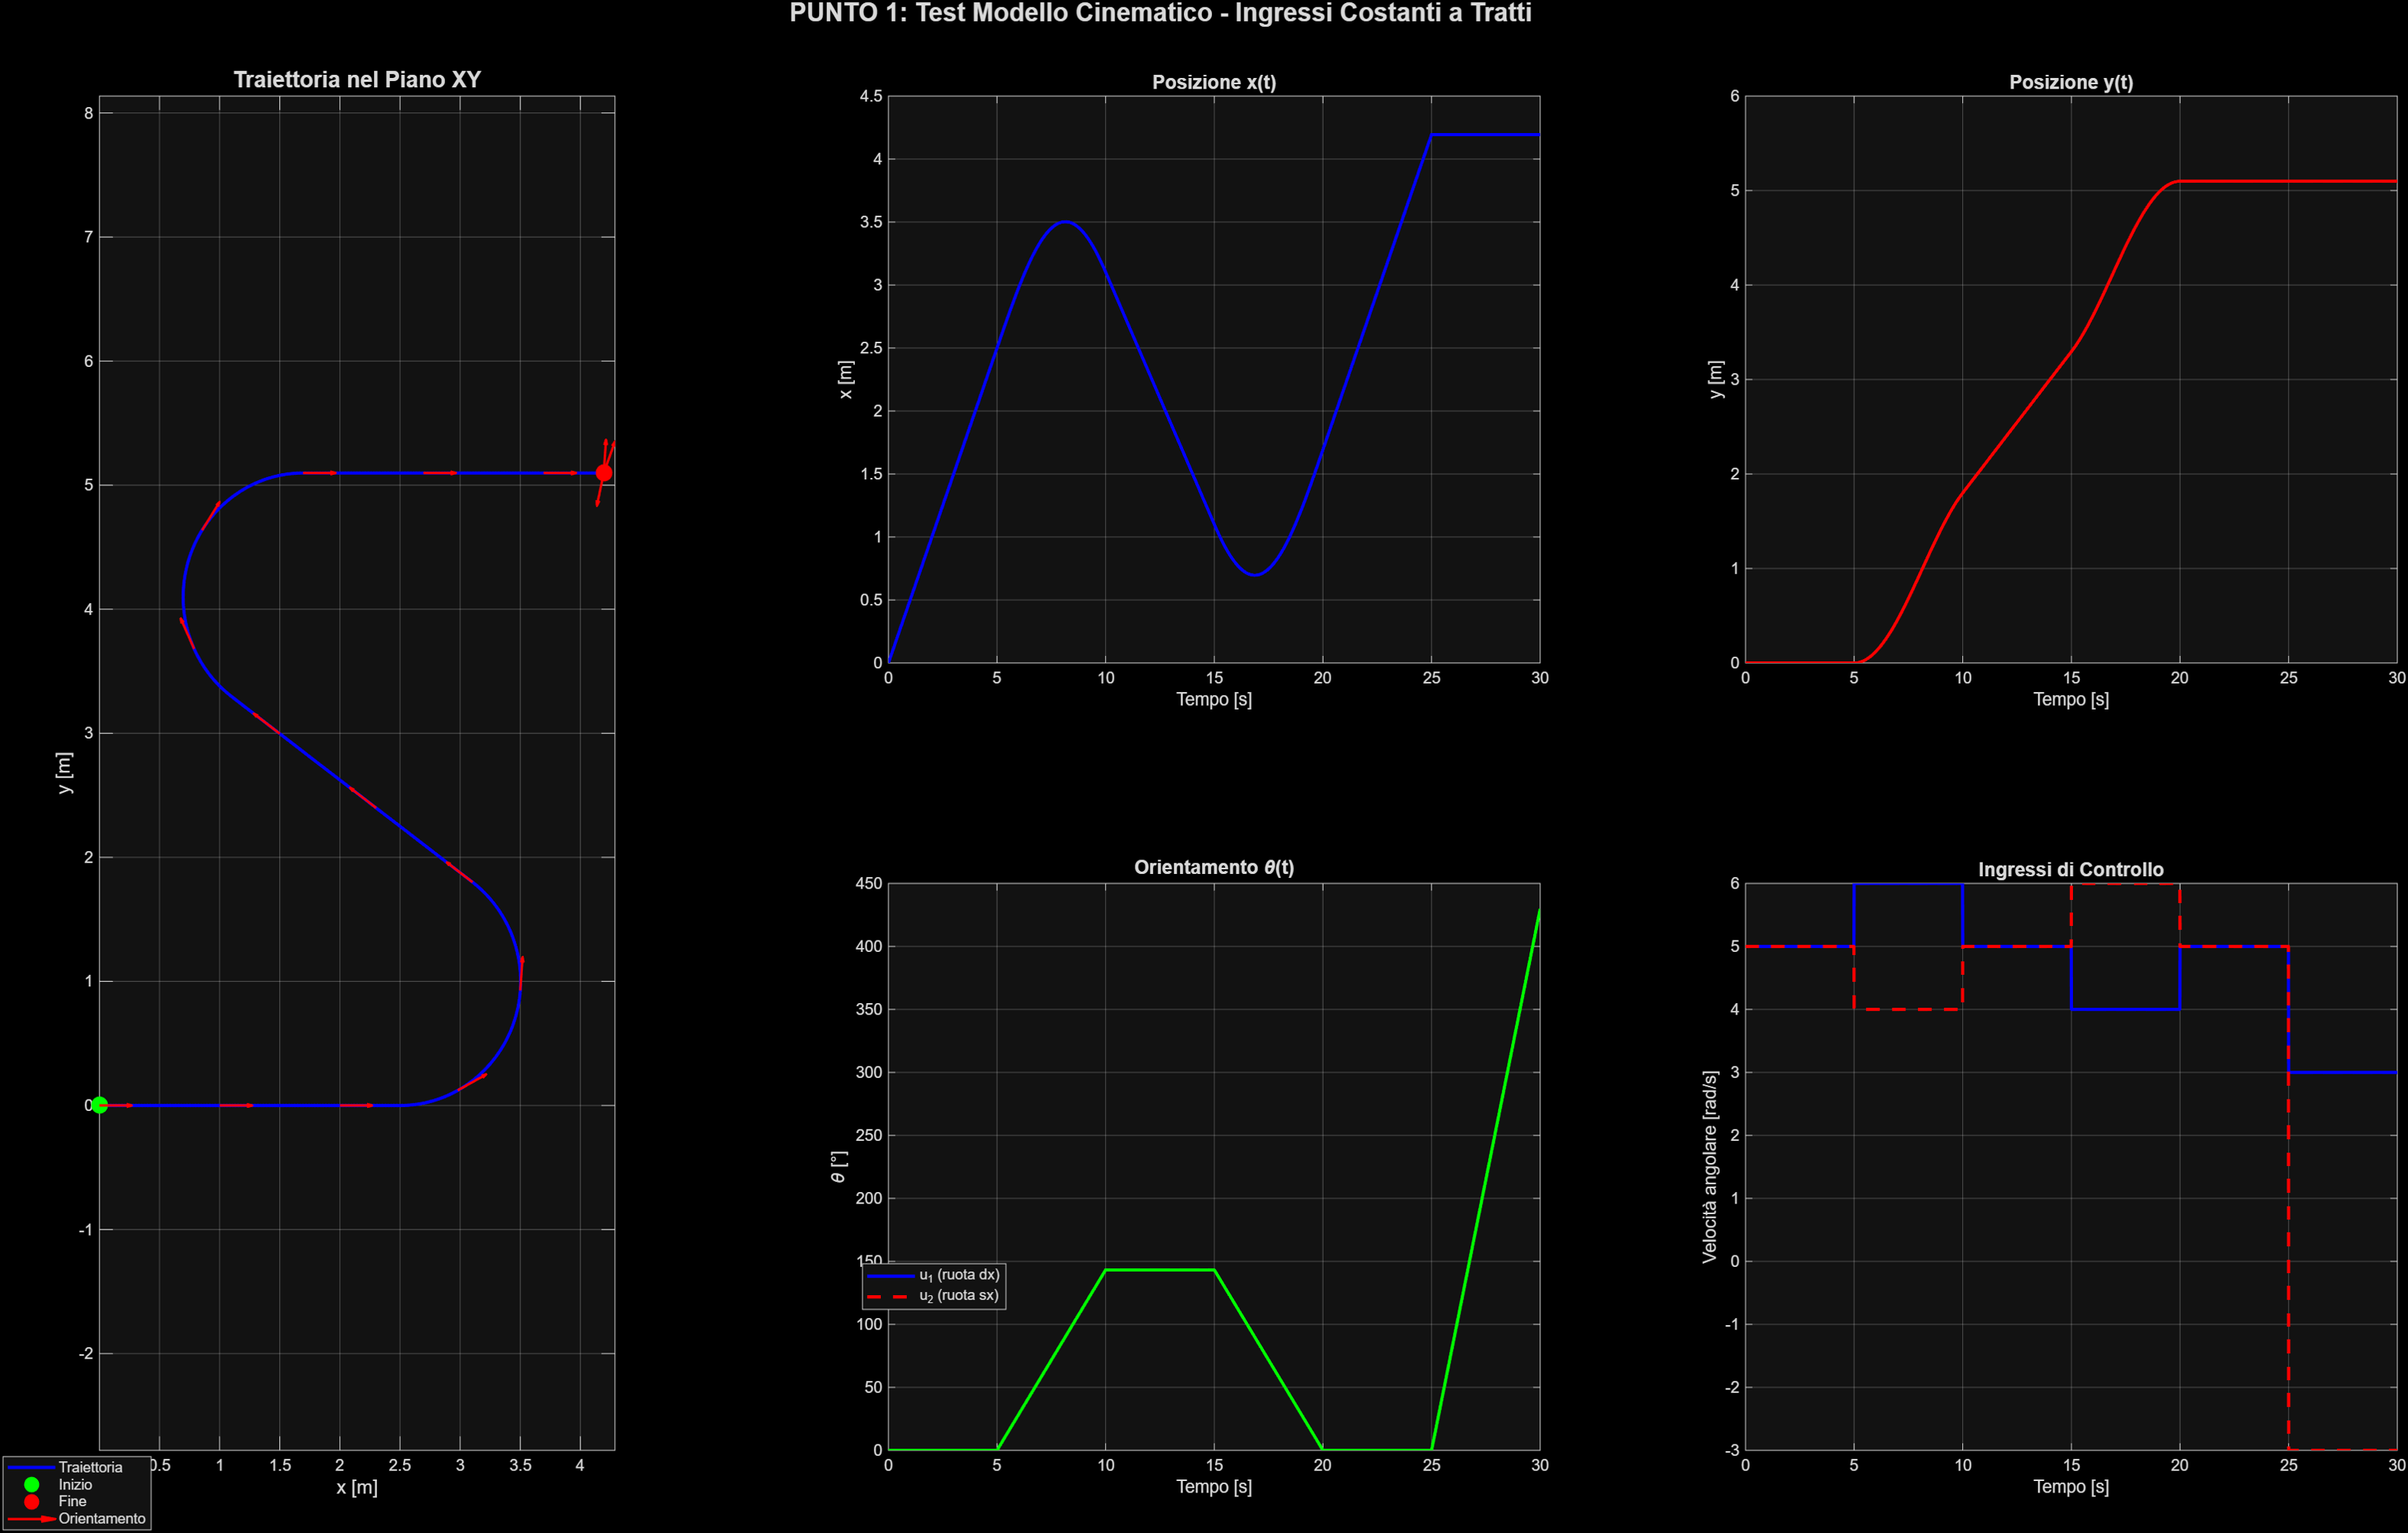
\includegraphics[width=1.0\textwidth]{chapter9/images/Punton1.png}
    \caption{Risultati del Punto 1: Traiettoria, evoluzione delle variabili di stato e profili degli ingressi di controllo.}
    \label{fig:p1_results}
\end{figure}


\newpage

\section{Conclusioni Punto 1}
Il modello cinematico è stato validato con successo. La corrispondenza tra gli ingressi applicati e lo stato finale \( z(T) \) dimostra che le matrici \( g_1(z) \) e \( g_2(z) \) descrivono correttamente la fisica dell'uniciclo. Il sistema è pronto per l'implementazione degli algoritmi di controllo e diagnosi guasti.